% SPDX-License-Identifier: AGPL-3.0-only
% Two-column IEEEtran manuscript of the user-level Coordinated Lunar Time error budget.
% PRIVATE (kshana-pro). Compile: tectonic main.tex   (or pdflatex x2)
% Numbers reproduce the committed P3 budget: lunar_time_budget.csv (tau sweep) and
% the P3 Table 1 realization budget (ledger oracle
% 0.009/0.035/0.901/0.995/1.732/50.035/151.238 ns), produced by the kshana-pro
% lunar-time-budget study composing the open kshana::powerlaw / kshana::holdover /
% kshana::allan / kshana::timetransfer / kshana::lunar_time closed forms.
% Figure: figures/make_figures.py (reads the committed CSV; reproducible by hand).
%
% This manuscript is a neutral, results-first reframe of an earlier branded report
% ("Realizing Coordinated Lunar Time at a User Is Frame-Limited, Not Clock-Limited")
% declined by arXiv moderation. Content and numbers are unchanged; framing is academic.
\documentclass[conference]{IEEEtran}
\usepackage{graphicx}
\usepackage{booktabs}
\usepackage{amsmath}
\usepackage{url}
\graphicspath{{figures/}}

\begin{document}

\title{A User-Level Error Budget for Realizing\\
Coordinated Lunar Time: Frame-Realization\\
versus Clock-Stability Contributions}

\author{\IEEEauthorblockN{Chakshu Baweja}
\IEEEauthorblockA{Ashforde O\"U \\ contact@ashforde.org}}

\maketitle

\begin{abstract}
A Coordinated Lunar Time (LTC) is being defined so that lunar users share a common
timescale, and the natural assumption is that realizing it to the nanosecond level
that lunar positioning needs is a clock problem. We assemble a user-level error
budget that shows it is not. Placing the candidate contributions on one axis, the
timing error at an averaging time of one day, we find that the terms which meet a
$1$ ns requirement are a ground optical master clock ($0.009$ ns), optical two-way
time transfer ($0.035$ ns), a post-processed lunar frame/ephemeris ($0.90$ ns), and
a space passive hydrogen maser ($0.99$ ns), while the terms that miss it are the
\emph{real-time} frame/ephemeris knowledge ($\sim$$50$ ns, the $\sim$$15$ m
real-time position budget expressed as light time) and a SWaP-limited $500$ g
miniRAFS ($\sim$$151$ ns/day). The binding constraint on a user realizing LTC is
therefore the \emph{real-time realization of the reference frame}, not the atomic
clock: a $50$-fold gap separates real-time from post-processed frame knowledge, and
no attainable clock closes it. We make the honesty boundary explicit: the clock
Allan-deviation synthesis and the quadrature assembly are Validated closed forms
over cited specifications, while the link floors, the frame-knowledge magnitudes,
and the relativistic residuals are Imported or Modelled allocations, and the
frame-limited conclusion inherits that modelled frame budget. We also show, by
sweeping the averaging time, that the frame-limited regime is not a single-$\tau$
artifact: a clock-versus-frame crossover occurs near $\tau^\ast\approx1.0$ day, and
the conclusion is invariant across a $1$--$5$ ns requirement band. The roadmap
implication is that the highest-leverage investment is real-time frame/ephemeris
prediction, an estimation problem, rather than further clock improvement. The engine
and the committed budget are open under AGPL-3.0.
\end{abstract}

\section{Introduction}
The lunar programs now under way require a common time. NASA, ESA, and their
partners, and at the policy level the 2024 direction to define a Coordinated Lunar
Time \cite{ltcpolicy}, are converging on an LTC realized through a network of clocks
and time-transfer links, much as Coordinated Universal Time is realized on Earth
\cite{iaulctime,ashby2024,bourgoin2026}. Lunar positioning to the metre level, the
target of the emerging navigation services, needs that time good to about a
nanosecond at the user, because a nanosecond of time error is $0.3$ m of ranging
error.

The intuitive reading is that meeting a $1$ ns budget is a matter of flying a good
enough clock. This paper tests that reading with a systems error budget and finds it
false. A user does not consume a clock in isolation: it consumes a clock \emph{plus}
the time-transfer link that ties the clock to LTC \emph{plus} the knowledge of the
reference frame and ephemeris in which its position, and hence its light-time
correction, is expressed. When all three are placed on a single axis, the timing
error each contributes at a one-day averaging time, the dominant term is not the
clock. It is the \emph{real-time} knowledge of the lunar frame and ephemeris, which
enters as a position uncertainty converted to time by light travel, and which no
clock choice removes.

We make three contributions of graded strength. \textbf{First, the budget
(Section~\ref{sec:method}--\ref{sec:results}).} We assemble seven contributions as
timing errors at $\tau=1$ day and sort them against the $1$ ns line
(Table~\ref{tab:budget}, Figure~\ref{fig:budget}). \textbf{Second, the conclusion
(Section~\ref{sec:frame}).} The real-time frame/ephemeris term ($\sim$$50$ ns)
dominates, a $50$-fold gap above the post-processed frame ($0.90$ ns) and roughly
$50\times$ the best clock, so the realization is frame-limited, not clock-limited.
\textbf{Third, the robustness (Section~\ref{sec:robust}).} A $\tau$-sweep shows the
crossover between the frame-dominated and clock-dominated regimes lies near one day,
so the conclusion is not a single-$\tau$ artifact, and it is invariant across a
$1$--$5$ ns requirement band. Throughout we tag each term Validated (a cross-checked
closed form over a cited spec) or Modelled/Imported (a budget allocation), because
the load-bearing conclusion rests on a modelled frame allocation and honesty about
that is the point.

\section{Related work}
\textbf{Lunar time scales.} The relativistic definition of a lunar timescale and its
rate relative to Terrestrial Time are set out by Ashby and Patla \cite{ashby2024},
Bourgoin et al. \cite{bourgoin2026}, and the IAU framework for a lunar celestial
reference system \cite{iaulctime}; the policy direction to realize an LTC is recent
\cite{ltcpolicy}. These fix the \emph{definition}; our subject is the error in a
user \emph{realizing} it.

\textbf{Clock stability.} The Allan deviation \cite{allan,riley} characterises an
oscillator, and its accumulated phase over an interval follows from the noise power
spectral densities. We use the standard three-term power-law model (white-FM,
flicker floor, random-walk-FM) calibrated to published specifications of a ground
optical master clock \cite{origlia2015}, a space passive hydrogen maser, a rubidium
atomic frequency standard, and a $500$ g miniature RAFS.

\textbf{Time transfer.} Earth--Moon two-way time transfer at radio frequency is
$\sim$$1$ ns class; optical two-way transfer reaches the few-to-tens-of-picoseconds
class \cite{twoway}. We enter these as link floors rather than deriving them.

\textbf{Frame and ephemeris.} The lunar ephemeris and reference frame are realized
from tracking; the post-processed (smoothed, fitted) solution is far better than the
real-time (predicted) one, and DE440 \cite{de440} and lunar laser ranging set the
achievable accuracies. The real-time-versus-post-processed gap is the crux of this
paper and the hand-off to a companion analysis of the real-time frame as an
Earth-orientation prediction problem \cite{baweja2026eop}.

\section{Method: the realization error budget}
\label{sec:method}
\textbf{The budget.} We treat the user's realized-time error as the quadrature sum
of independent contributions,
\begin{equation}
x_\Sigma(\tau) = \sqrt{\textstyle\sum_i x_i^2(\tau)},
\label{eq:rss}
\end{equation}
each $x_i$ a timing error at averaging time $\tau$. A user picks one clock, one
time-transfer link, and inherits the frame/ephemeris term; \eqref{eq:rss} combines
that chosen configuration. Table~\ref{tab:budget} instead lists the candidate terms
side by side at $\tau=1$ day, so the comparison is per-component: which candidate, on
its own, meets or misses $1$ ns.

\textbf{Clock term.} The clock contributes $x_{\mathrm{clock}}(\tau) =
\sigma_y(\tau)\,\tau$, with the fractional-frequency stability from the three-term
power-law Allan variance
\begin{equation}
\sigma_y^2(\tau) = \frac{h_0}{2\tau} + 2\ln 2\, h_{-1}
+ \frac{2\pi^2}{3}h_{-2}\,\tau,
\label{eq:adev}
\end{equation}
(white-FM $\tau^{-1/2}$, flicker floor, random-walk-FM $\tau^{+1/2}$), each clock's
$h$-coefficients calibrated so $\sigma_y(\tau)$ reproduces its published spec. At
$\tau=1$ day this gives $0.009$ ns for a ground optical master, $0.99$ ns for a space
PHM, and $151$ ns for the SWaP-limited miniRAFS.

\textbf{Link term.} The Earth--Moon two-way time-transfer floor enters directly:
$1.732$ ns for the RF class and $0.035$ ns for the optical class.

\textbf{Frame term.} The frame/ephemeris knowledge enters as a position uncertainty
converted to time by light travel, $x_{\mathrm{frame}} = \delta r / c$. A real-time
position budget of $\sim$$15$ m gives $50.035$ ns; the post-processed budget of
$\sim$$0.27$ m gives $0.901$ ns.

\textbf{Deterministic relativistic terms, for scale.} The secular TT-to-lunar-time
drift is $\sim$$1469$ ns/day and the topographic redshift spread across lunar surface
elevations is $\sim$$26$ ns/day \cite{ashby2024,bourgoin2026}; these are deterministic
and removed by the timescale definition, shown here for scale and not summed into the
stochastic budget. A small relativistic \emph{residual} ($\sim$$0.05$ ns) is carried.

\section{Results}
\label{sec:results}
Table~\ref{tab:budget} is the budget, sorted. Four terms meet $1$ ns and three miss
it. The three that miss are the RF two-way link ($1.732$ ns, marginally over), the
real-time frame/ephemeris ($50.035$ ns), and the miniRAFS ($151.238$ ns/day). The
optical master clock, optical transfer, post-processed frame, and space PHM all meet
it. Figure~\ref{fig:budget}(a) shows the same result as a sorted bar chart against
the requirement.

\begin{table}[t]
\centering
\caption{Seven-term LTC realization error budget at $\tau=1$ day, sorted. Meets-$1$ns
column marks each candidate. Provenance: clock synthesis and the quadrature assembly
Validated; link floors, frame magnitudes, and relativistic residual Modelled/Imported.}
\label{tab:budget}
% Tightened from the 6pt default: at the default this table runs 7.7pt past the
% column and TeX reports an overfull hbox, which on an external recompile (arXiv's)
% prints as text bleeding into the gutter. 4pt clears it without shrinking the type.
\setlength{\tabcolsep}{4pt}
\begin{tabular}{lrcl}
\toprule
Contribution & Error & $\leq 1$ ns & Provenance \\
\midrule
Ground optical master clock   & $0.009$ ns  & yes & Validated \\
Optical two-way transfer      & $0.035$ ns  & yes & Modelled \\
Post-processed frame/eph.\    & $0.901$ ns  & yes & Modelled \\
Space PHM                     & $0.995$ ns  & yes & Validated \\
RF two-way transfer           & $1.732$ ns  & no  & Modelled \\
Real-time frame/ephemeris     & $50.035$ ns & no  & Modelled \\
$500$ g miniRAFS              & $151.238$ ns& no  & Validated \\
\bottomrule
\end{tabular}
\end{table}

\begin{figure}[t]
\centering
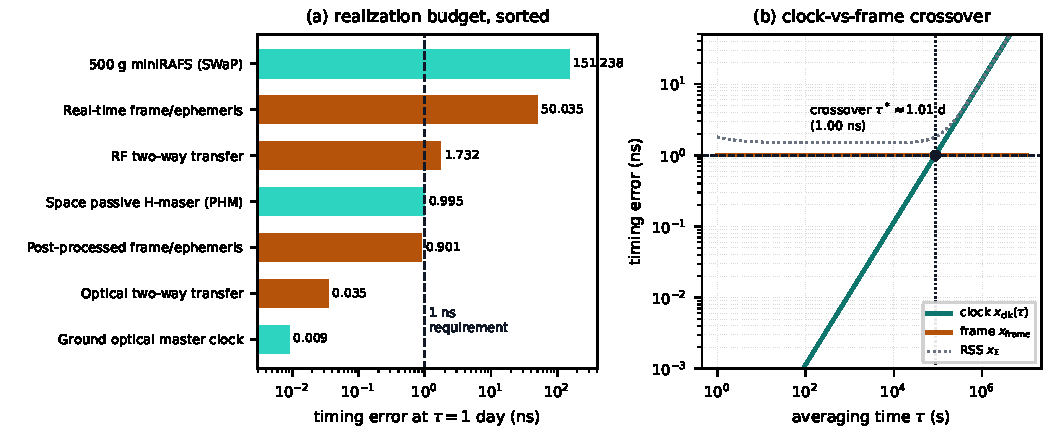
\includegraphics[width=\columnwidth]{fig1_ltc_budget.pdf}
\caption{(a) The seven-term realization budget at $\tau=1$ day, sorted, against the
$1$ ns requirement (dashed); teal bars are Validated clock terms, brass are
Modelled link/frame allocations. (b) For a chosen configuration (passive H-maser),
the rising clock term $x_{\mathrm{clk}}(\tau)$ and the constant frame term
$x_{\mathrm{frame}}$ from the committed \texttt{lunar\_time\_budget.csv} cross at
$\tau^\ast\approx1.0$ day ($\approx1.0$ ns); the RSS $x_\Sigma$ is dotted. The
frame-limited regime is not a single-$\tau$ artifact.}
\label{fig:budget}
\end{figure}

\section{The realization is frame-limited, not clock-limited}
\label{sec:frame}
The dominant systematic is the real-time frame/ephemeris term at $\sim$$50$ ns. It is
$\sim$$50\times$ the post-processed frame ($0.90$ ns) and $\sim$$50\times$ the best
clock, and it is not removed by any clock choice: flying a better oscillator moves a
term that is already below $1$ ns and leaves the $50$ ns term untouched. The lever
that matters is therefore the \emph{real-time realization of the frame and
ephemeris}, the difference between what is known about a lunar vehicle's position in
real time ($\sim$$15$ m) and what is reconstructed after the fact ($\sim$$0.27$ m).
This is an estimation and prediction problem, not a metrology one: it is set by how
well the lunar orbit and Earth-orientation state can be \emph{predicted} over the
real-time latency, which we take up separately \cite{baweja2026eop}. The practical
consequence for a lunar PNT architecture is a reallocation of effort: the marginal
nanosecond is bought far more cheaply by improving real-time ephemeris prediction and
frame realization than by improving the clock, which for realistic clocks is already
not the binding term.

\section{Robustness: the crossover is near one day}
\label{sec:robust}
A single-$\tau$ budget invites the objection that the term ordering is an artifact of
the chosen averaging time: a clock term grows with $\tau$ while the frame term is
constant, so at some $\tau$ the clock must overtake the frame. We therefore sweep
$\tau$ and locate the crossover. Figure~\ref{fig:budget}(b) plots the clock term
$x_{\mathrm{clk}}(\tau)$ and the constant frame term $x_{\mathrm{frame}}$ for a
passive-H-maser configuration from the committed budget; the frame term dominates
until the growing clock term overtakes it at $\tau^\ast\approx8.7\times10^{4}$ s
($\approx1.0$ day), where the two are equal at $\approx1.0$ ns, in the flicker-floor
regime. For the operationally relevant
averaging times at or below a day, the budget is frame-dominated. The crossover
identity is a closed form ($\tau^\ast\!\cdot\!\mathrm{floor}=\delta r/c$ for a
flicker-floor clock), checked against an analytic oracle to machine precision, so the
crossover location is Validated even though the frame magnitude that sets it is
Modelled. The frame-not-clock conclusion is invariant across a $1$--$5$ ns
requirement band: at every requirement in that band the real-time frame term is above
the line and the clock terms (for the optical master and PHM) are below it.

\section{Limitations and honesty boundary}
\label{sec:honesty}
We state the limits precisely.

\textbf{One Validated claim, cleanly bounded.} What is Validated is the computational
pipeline: the three-term power-law Allan synthesis \eqref{eq:adev} reproduces the
cited clock specs, and the quadrature assembly \eqref{eq:rss} and the crossover
identity are closed forms checked against analytic oracles. The clock rows for the
optical master, PHM, and miniRAFS inherit this and are Validated over their cited
specifications.

\textbf{The link, frame, and relativistic magnitudes are Modelled.} The RF/optical
two-way floors, the $\sim$$15$ m real-time and $\sim$$0.27$ m post-processed position
budgets, and the relativistic residual are documented budget allocations, not
independently derived here. They are caller-overridable, and the RSS total and the
crossover $\tau^\ast$ \emph{value} inherit that modelled frame allocation.

\textbf{The headline conclusion inherits a modelled term.} The frame-limited
conclusion rests on the real-time frame/ephemeris budget being $\sim$$50\times$ the
post-processed one. That $50\times$ lever is a Modelled allocation; deriving the
real-time position-error growth endogenously, by propagating a lunar orbit-
determination and frame-realisation covariance through the prediction latency, is the
companion analysis \cite{baweja2026eop} and would lift this term from Modelled to
Validated. Until then, the conclusion is a Modelled result stated as such.

\textbf{Per-component, not a single score.} We report the budget as a per-term matrix
against the requirement, never collapsed to one aggregate number, so a reader can see
which term dominates and at what $\tau$. The deterministic relativistic terms are
shown for scale and excluded from the stochastic RSS.

\section{Conclusion}
Realizing Coordinated Lunar Time at a user to the nanosecond level that lunar
positioning needs is, on a systems error budget, limited by the real-time
realization of the reference frame and ephemeris, not by the atomic clock. At a
one-day averaging time the real-time frame term ($\sim$$50$ ns) dominates a budget
in which the best clocks, the optical two-way link, and even the post-processed
frame already meet $1$ ns; the gap between real-time and post-processed frame
knowledge is $\sim$$50\times$, and no attainable clock closes it. A $\tau$-sweep puts
the clock-versus-frame crossover near one day, so the conclusion holds across the
operationally relevant averaging times and a $1$--$5$ ns requirement band. We were
explicit that the clock synthesis and the quadrature assembly are Validated closed
forms while the link, frame, and relativistic magnitudes are Modelled allocations,
and that the headline conclusion inherits the modelled frame budget pending an
endogenous derivation \cite{baweja2026eop}. The roadmap implication is direct: for a
lunar PNT architecture, the marginal investment belongs in real-time ephemeris
prediction and frame realization, not in the clock. The engine and the committed
budget are open under AGPL-3.0.

\section*{Reproducibility}
The clock Allan synthesis \eqref{eq:adev}, the quadrature assembly \eqref{eq:rss},
the light-time conversion, and the crossover identity are closed forms in the open
Kshana simulator \cite{kshana} (\texttt{kshana::powerlaw}, \texttt{kshana::holdover},
\texttt{kshana::allan}, \texttt{kshana::timetransfer}, \texttt{kshana::lunar\_time})
under AGPL-3.0. The kshana-pro lunar-time-budget study emits the committed
\texttt{lunar\_time\_budget.csv} (byte-stable, scenario-hash pinned) that
regenerates the Table~\ref{tab:budget} numbers
($0.009/0.035/0.901/0.995/1.732/50.035/151.238$ ns) and the $\tau$-sweep;
\texttt{figures/make\_figures.py} reads that CSV and prints the crossover
cross-check ($\tau^\ast\approx1.006$ day, $x^\ast\approx1.001$ ns).

\begin{thebibliography}{99}
\bibitem{ltcpolicy} Executive Office of the President, Office of Science and
Technology Policy, ``Celestial Time Standardization in Support of the National
Cislunar Science \& Technology Strategy,'' policy memorandum, 2024.

\bibitem{iaulctime} International Astronomical Union, ``Resolution on the definition
of a lunar celestial reference system and lunar coordinate time,'' IAU, 2024.

\bibitem{ashby2024} N.~Ashby and B.~Patla, ``Relativistic effects in the definition
and realization of a lunar time scale,'' \emph{The Astronomical Journal}, 2024.

\bibitem{bourgoin2026} A.~Bourgoin \emph{et al.}, ``Relativistic time transfer and
the realization of a lunar time scale,'' preprint, 2026.

\bibitem{allan} D.~W. Allan, ``Statistics of atomic frequency standards,''
\emph{Proc. IEEE}, vol.~54, no.~2, pp.~221--230, 1966.

\bibitem{riley} W.~J. Riley, \emph{Handbook of Frequency Stability Analysis},
NIST Special Publication 1065. Boulder, CO: National Institute of Standards and
Technology, 2008.

\bibitem{origlia2015} S.~Origlia \emph{et al.}, ``Development of a strontium
optical lattice clock for the SOC mission on the ISS,'' \emph{Proc. SPIE}, 2015.

\bibitem{twoway} I.~Prochazka \emph{et al.}, ``Laser time transfer and its
application in space,'' review of two-way optical/RF Earth--space time transfer,
\emph{Metrologia}, 2017.

\bibitem{de440} R.~S. Park, W.~M. Folkner, J.~G. Williams, and D.~H. Boggs, ``The
JPL planetary and lunar ephemerides DE440 and DE441,'' \emph{The Astronomical
Journal}, vol.~161, no.~3, art.~105, 2021.

\bibitem{baweja2026eop} C.~Baweja, ``The lunar real-time frame gap is an
Earth-orientation prediction problem,'' preprint, 2026.

\bibitem{kshana} C.~Baweja, ``Kshana: an open, reproducible PNT-resilience
simulator,'' software, AGPL-3.0-only, 2026. [Online]. Available:
\url{https://github.com/ashfordeOU/kshana}
\end{thebibliography}

\end{document}
